\chapter{Preliminaries}

\section{Course Resources}

\refb{Course Resources}{
    \begin{itemize}
        \item The textbook, \textit{Mathematics for Machine Learning}, to be referenced as Deisenroth et al. (2020), can be found \href{https://mml-book.github.io/book/mml-book.pdf}{here}

        \item The textbook, \textit{Machine Learning a Probabilistic Perspective}, to be referenced as Murphy (2012), can be found \href{https://raw.githubusercontent.com/kerasking/book-1/master/ML\%20Machine\%20Learning-A\%20Probabilistic\%20Perspective.pdf}{here}

        \item The textbook, \textit{Pattern Recognition and Machine Learning}, to be referenced as Bishop (2006), can be found \href{https://www.microsoft.com/en-us/research/uploads/prod/2006/01/Bishop-Pattern-Recognition-and-Machine-Learning-2006.pdf}{here}
    \end{itemize}
}


\refb{Additional Resources}{
    \begin{itemize}
        \item \textbf{Linear Algebra:} Chapter 2 (page 29) \textit{Bengio et al. (2017)}
              \href{https://www.deeplearningbook.org/contents/linear_algebra.html}{link}

        \item \textbf{Probability Theory Review:} Chapter 2 (page 27) \textit{Murphy (2012)}. \textit{Machine learning: a probabilistic perspective}. MIT Press.

        \item \textbf{Calculus Review:} Chapter 5 (page 139) \textit{Deisenroth et al. (2020)}. \textit{Mathematics for machine learning}. Cambridge University Press.
    \end{itemize}
}




\section{Course Notation}

Real values are denoted with lower-case Roman letters, e.g. $x$, $y$, $z$. As convention, we will use a bold Roman letter or a Greek symbol to denote a vector, e.g. $\bm{x}$, $\boldsymbol{\theta}$.

Do not confuse this with random variables, which are denoted using bold, non-italic Roman letters, e.g. $\mathbf{x}$, $\mathbf{y}$, $\mathbf{z}$. Matrices are represented by upper-case Roman letters such as $X$ or random matrices like $\mathbf{X}$. Greek letters will always have their type specified, except for $\boldsymbol{\theta}$, which will be used without loss of generality to represent model parameters.




\[
    \boldsymbol{\theta} = \begin{bmatrix}
        \theta_1 \\ \vdots \\ \theta_n
    \end{bmatrix}
    \quad
    \mb{x} = \begin{bmatrix}
        x_1 \\ \vdots \\ x_n
    \end{bmatrix}
\]


\begin{table}[h!]
    \centering
    \begin{tabularx}{\textwidth}{@{}X X@{}}
        \toprule
        \textbf{Notation Type} & \textbf{Example}                                                                        \\ \midrule
        Real Values            & $x$, $y$, $z$                                                                           \\
        Vectors                & $\bm{x}$, $\boldsymbol{\theta}$ (where $\boldsymbol{\theta}$ represents parameters) \\
        Random Variables       & $\mathbf{x}$, $\mathbf{y}$, $\mathbf{z}$                                                \\
                               & Example: $\mathbf{z} \sim \text{Unif}(0, 1)$                                            \\
        Matrices               & $X = \begin{pmatrix} x_{11} & x_{12} \\ x_{21} & x_{22} \end{pmatrix}$                  \\
        Random Matrices        & $\mathbf{X}$                                                                            \\
                               & Example: $\mathbf{X} \sim \mathcal{N}(\mathbf{0}, \mathbf{I})$                          \\ \bottomrule
    \end{tabularx}
    \caption{Summary of Course Notation with Examples}
\end{table}






\section{Linear Algebra}
A core prerequisite for this class is linear algebra. Please use this section and references herein to brush up on necessary concepts.
\subsection{Vectors}

A vector is defined by a list of numbers. It is most useful to geometrically interpret vectors as points in space.

\begin{equation}
    \bm{x} := \begin{bmatrix} x_1 \\ x_2 \\ \vdots \\ x_n \end{bmatrix}
\end{equation}
\subsection{Vectors Operations}

We have several vector operations:
\begin{itemize}
    \item \textbf{Scalar Multiplication}:
          \begin{equation}
              \alpha \bm{x} = \begin{bmatrix} \alpha x_1 \\ \alpha x_2 \\ \vdots \\ \alpha x_n \end{bmatrix}
          \end{equation}

    \item \textbf{Vector Addition}:
          \begin{equation}
              \bm{x} + \bm{y} = \begin{bmatrix} x_1 + y_1 \\ x_2 + y_2 \\ \vdots \\ x_n + y_n \end{bmatrix}
          \end{equation}

    \item \textbf{Dot Product}:
          \begin{equation}
              \bm{x} ^\top \bm{y} = \sum^n_{i=1} x_i y_i
          \end{equation}
\end{itemize}

% Table for vector notation
\begin{table}[h!]
    \centering
    \begin{tabularx}{\textwidth}{@{}p{\dimexpr\textwidth/3-2\tabcolsep} X@{}}
        \toprule
        \textbf{Symbol}                       & \textbf{Meaning}                                           \\ \midrule
        $\mb{v}^\top$                         & Transpose of $\mb{v}$                                      \\
        $\mb{u}^\top \mb{v}$                  & Inner (scalar) product                                     \\
        $\mb{u} \mb{v}^\top$                  & Outer product (n $\times$ n matrix)                        \\
        $\mb{u} \odot \mb{v}$                 & Hadamard/Elementwise product, $[u_1 v_1, \ldots, u_n v_n]$ \\
        $\text{dim}(\mb{v})$                  & Dimensionality of $\mb{v}$ (namely $n$)                    \\
        $\text{diag}(\mb{v})$                 & Diagonal $n \times n$ matrix made from vector $\mb{v}$     \\
        $1 \text{ or } \mb{1}_n$              & Vector of ones (of length $n$)                             \\
        $0 \text{ or } \mb{0}_n$              & Vector of zeros (of length $n$)                            \\
        $\|\mb{v}\| \text{ or } \|\mb{v}\|_2$ & Euclidean or $\ell_2$ norm, $\sqrt{\sum_{i=1}^{n} v_i^2}$  \\
        $\|\mb{v}\|_1$                        & $\ell_1$ norm, $\sum_{i=1}^{n} |v_i|$                      \\
        $\mb{e}_i$                            & $i$th-basis vector (1 in dimension $i$ and 0 elsewhere)    \\ \bottomrule
    \end{tabularx}
    \caption{Standard Notation for Vectors}
\end{table}

\subsection{Matrices}

Matrices define linear transforms. Geometrically, it is best to interpret them as transformations whose columns are the new basis vectors.

\begin{equation}
    A := \begin{bmatrix} A_{1,1} & A_{1,2} & \cdots & A_{1,n} \\ A_{2,1} & A_{2,2} & \cdots & A_{2,n} \\ \vdots & \vdots & \ddots & \vdots \\ A_{m,1} & A_{m,2} & \cdots & A_{m,n} \end{bmatrix} \quad A \in \mathbb{R}^{m \times n}
\end{equation}


Non-square matrices can be thought of as transformations from $\mathbb{R}^m$ dimentional space to $\mathbb{R}^n$ dimensional space.

\subsection{Matrix Operations}

We define several matrix operations as follows:

\begin{itemize}
    \item \textbf{Scalar Multiplication}:
          \begin{equation}
              cA = c A_{i,j}
          \end{equation}

    \item \textbf{Hadamard Product (Element-wise Multiplication)}:
          \begin{equation}
              A \circ B = A_{i,j} B_{i,j}
          \end{equation}

    \item \textbf{Matrix Subtraction}:
          \begin{equation}
              A - B = A_{i,j} - B_{i,j}
          \end{equation}

    \item \textbf{Matrix Product}:
          \begin{equation}
              C_{i,j} = \sum_{k} A_{i,k} B_{k,j}
          \end{equation}

    \item \textbf{Trace of a Matrix}:
          \begin{equation}
              \text{Tr}(A) = \sum_{i} A_{i,i}
          \end{equation}

    \item \textbf{Kronecker Product}:
          \begin{equation}
              A \otimes B =
              \begin{pmatrix}
                  a_{11} B & a_{12} B & \dots  & a_{1n} B \\
                  a_{21} B & a_{22} B & \dots  & a_{2n} B \\
                  \vdots   & \vdots   & \ddots & \vdots   \\
                  a_{m1} B & a_{m2} B & \dots  & a_{mn} B
              \end{pmatrix}
          \end{equation}
          The Kronecker product $A \otimes B$ results in a block matrix, where each element $a_{ij}$ of matrix $A$ is multiplied by the entire matrix $B$.

    \item \textbf{Positive Definite Matrix} ($S \succ 0$):
          \begin{equation}
              \mathbf{x}^\top S \mathbf{x} > 0 \quad \forall \, \mathbf{x} \in \mathbb{R}^n, \, \mathbf{x} \neq \mathbf{0}
          \end{equation}
          A matrix $S$ is positive definite if for all non-zero vectors $\mathbf{x}$, the quadratic form $\mathbf{x}^\top S \mathbf{x}$ is strictly greater than 0. Positive definite matrices are often used to indicate that a matrix represents a convex function.
\end{itemize}


\textbf{Dimensional Notation}:
\begin{equation}
    A \in \mathbb{R}^{n \times m} : \mathbb{R}^n \to \mathbb{R}^m
\end{equation}
\begin{equation}
    B \in \mathbb{R}^{m \times k} : \mathbb{R}^m \to \mathbb{R}^k
\end{equation}
\begin{equation}
    AB \in \mathbb{R}^{n \times k} : \mathbb{R}^n \to \mathbb{R}^k
\end{equation}



\sn{Matrix Multiplication as Dot Products of the Row and Column}{
    This matrix multiplication is equivalent to the dot product between row \( i \) of matrix \( A \) and column \( j \) of matrix \( B \):
    \begin{equation}
        \mb{x}^\top \mb{y} = \sum_{i=1}^{n} x_i y_i
    \end{equation}
}



% Table for matrix notation
\begin{table}[h!]
    \centering
    \begin{tabularx}{\textwidth}{@{}p{\dimexpr\textwidth/3-2\tabcolsep} X@{}}
        \toprule
        \textbf{Symbol}               & \textbf{Meaning}                                  \\ \midrule
        $\mb{X}_{:,j}$                & $j$-th column of matrix                           \\
        $\mb{X}_{i,:}$                & $i$-th row of matrix (treated as a column vector) \\
        $\mb{X}_{ij}$                 & Element $(i, j)$ of matrix                        \\
        $\mb{X}^\top$                 & Transpose of a matrix                             \\
        $\text{diag}(\mb{S})$         & Diagonal vector extracted from square matrix      \\
        $\mb{I} \text{ or } \mb{I}_n$ & Identity matrix of size $n \times n$              \\
        $\mb{X} \odot \mb{Y}$         & Hadamard/Elementwise product                      \\
        $\mb{X} \otimes \mb{Z}$       & Kronecker product                                 \\
        $\mb{S} \succ 0$              & True iff $\mb{S}$ is a positive definite matrix   \\
        $\text{tr}(\mb{S})$           & Trace of a square matrix                          \\
        $\text{det}(\mb{S})$          & Determinant of a square matrix                    \\
        $|\mb{S}|$                    & Determinant of a square matrix                    \\ \bottomrule
    \end{tabularx}
    \caption{Standard Notation for Matrices}
\end{table}

\section{Calculus}

In this section, we cover basic multivariate calculus and key identities. These are considered prerequisite material, so students should spend time reviewing them if needed. For a more in-depth refresher, refer to Chapter 5 of Deisenroth et al. (2020).

Unqualified, a \textbf{function} is a mapping from the reals to the reals: $f : \mathbb{R} \to \mathbb{R}$. The mapping of a value $x$ from the domain is denoted $f(x)$. The derivative is defined as:
\[
f'(x) = \frac{df}{dx} = \lim_{h \to 0} \frac{f(x+h) - f(x)}{h}
\]
assuming the limit exists. This is also known as the forward finite difference quotient.

\textbf{Leibniz} and \textbf{Lagrange} notations are often used for derivatives, as shown below:

\begin{table}[h]
    \centering
    \begin{tabularx}{\textwidth}{@{}lX@{}}
        \toprule
        \textbf{Notation Type} & \textbf{Representation} \\ \midrule
        Leibniz Notation & $\frac{dy}{dx}, \frac{d}{dx} f$ \\
        Lagrange Notation & $f'(x), f'(a)$ (for derivative at $a$) \\ \bottomrule
    \end{tabularx}
    \caption{Comparison of Leibniz and Lagrange Notations}
\end{table}

The notation $\frac{dy}{dx}\big|_{a}$ is used for the derivative of $f$ at $a$, while $f'(a)$ is used in Lagrange notation.

\section{Multivariate Calculus}

For vector-valued functions $f : \mathbb{R}^n \to \mathbb{R}$, we define the partial derivative:
\[
\frac{df}{dx_i} = \lim_{h \to 0} \frac{f(x + h e_i) - f(x)}{h}
\]
where $e_i$ is the $i$-th basis vector. This extends the definition of the derivative to each variable.

The gradient $\mathbf{g}$, or $\nabla f$, is defined as the collection of all partial derivatives into a row vector:
\[
\mathbf{g} = \nabla f = \left[ \frac{df}{dx_0}, \frac{df}{dx_1}, \dots, \frac{df}{dx_n} \right]
\]
The gradient maps vectors to vectors: $\mathbf{g} : \mathbb{R}^n \to \mathbb{R}^n$, which we call a \textbf{vector field}.

The derivative of a vector field $f : \mathbb{R}^n \to \mathbb{R}^m$ is a matrix called the \textbf{Jacobian}, given by:
\[
\nabla f = 
\begin{bmatrix}
    \frac{\partial f_1}{\partial x_1} & \frac{\partial f_1}{\partial x_2} & \dots & \frac{\partial f_1}{\partial x_n} \\
    \frac{\partial f_2}{\partial x_1} & \frac{\partial f_2}{\partial x_2} & \dots & \frac{\partial f_2}{\partial x_n} \\
    \vdots & \vdots & \ddots & \vdots \\
    \frac{\partial f_m}{\partial x_1} & \frac{\partial f_m}{\partial x_2} & \dots & \frac{\partial f_m}{\partial x_n} \\
\end{bmatrix}
\]
where $f_i$ represents the $i$-th output of the function $f$. This matrix captures all partial derivatives and forms the foundation for calculating Jacobians of vector-valued functions.

\section{Probability and Statistics}

$x$ is a sample from a random variable $X$. \\

\noindent $P(X=x)$ refers to probability that the random variable $X$ takes on the value $x$.

\subsection{Probability Density Function (PDF)}
\begin{marginfigure}[100pt]
    \centering
    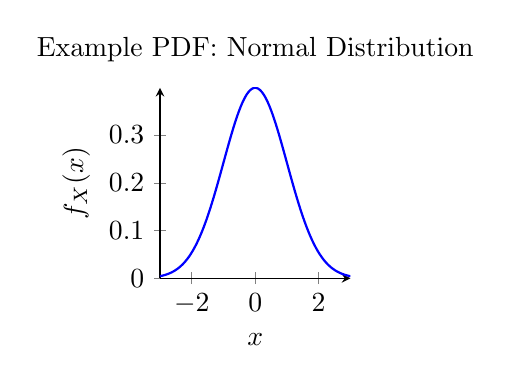
\begin{tikzpicture}
        \begin{axis}[
                width=4cm,
                height=4cm,
                xlabel={$x$},
                ylabel={$f_X(x)$},
                domain=-3:3,
                samples=100,
                axis lines=left,
                ymin=0,
                legend pos=north east,
                title={Example PDF: Normal Distribution}
            ]
            \addplot[blue, thick] {exp(-x^2 / 2) / sqrt(2 * pi)};
        \end{axis}
    \end{tikzpicture}
    \caption{Probability Density Function of a standard normal distribution}
\end{marginfigure}

The Probability Density Function (PDF) of a continuous random variable \(X\) is a function \(f_X(x)\) that describes the relative likelihood for this random variable to take on a given value. The PDF has the following properties:
\begin{itemize}
    \item \(f_X(x) \geq 0\) for all \(x\).
    \item \(\int_{-\infty}^{\infty} f_X(x) \, dx = 1\).
\end{itemize}

Mathematically, the PDF is defined such that the probability that \(X\) lies within a particular interval \([a, b]\) is given by:
\[
    P(a \leq X \leq b) = \int_{a}^{b} f_X(x) \, dx.
\]

The most common example of a PDF is the normal distribution, which is characterised by two parameters: the mean \(\mu\) and the variance \(\sigma^2\). The PDF of a normal distribution is given by:
\[
\mathcal{N}(x; \mu, \sigma^2) = \frac{1}{\sqrt{2\pi\sigma^2}} \exp\left(-\frac{(x - \mu)^2}{2\sigma^2}\right).  
\]


\subsection{Cumulative Distribution Function (CDF)}
\begin{marginfigure}[50pt]
    \centering
    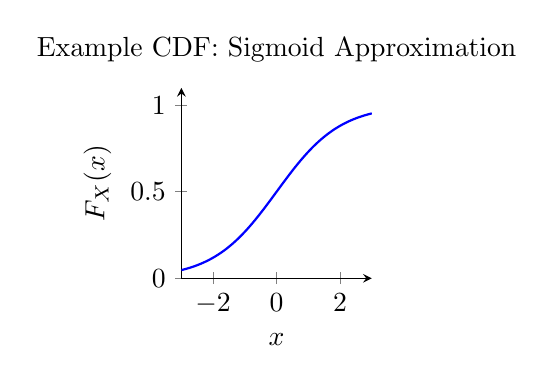
\begin{tikzpicture}
        \begin{axis}[
                width=4cm,
                height=4cm,
                xlabel={$x$},
                ylabel={$F_X(x)$},
                domain=-3:3,
                samples=100,
                axis lines=left,
                ymin=0, ymax=1.1,
                legend pos=south east,
                title={Example CDF: Sigmoid Approximation}
            ]
            \addplot[blue, thick] {1 / (1 + exp(-x))};
        \end{axis}
    \end{tikzpicture}
    \caption{Cumulative Distribution Function}
\end{marginfigure}

The Cumulative Distribution Function (CDF) of a continuous random variable \(X\) is a function \(F_X(x)\) that describes the probability that \(X\) will take a value less than or equal to \(x\). It is defined as:
\[
    F_X(x) = P(X \leq x) = \int_{-\infty}^{x} f_X(t) \, dt.
\]

The CDF has the following properties:
\begin{itemize}
    \item \(0 \leq F_X(x) \leq 1\) for all \(x\).
    \item \(F_X(x)\) is a non-decreasing function.
    \item \(\lim_{x \to -\infty} F_X(x) = 0\).
    \item \(\lim_{x \to \infty} F_X(x) = 1\).
\end{itemize}

\section{Moments}

Moments help describe probability distributions. The \textbf{first moment} is the mean (or centre of mass), the \textbf{second moment} is the variance (or spread), and the \textbf{third moment} is the skewness. Higher moments are also useful but are less common in practice.

The \textbf{expectation} of a distribution, or its first moment, is given by:
\[
\mu = \mathbb{E}[x] = \int_{-\infty}^{\infty} p(x = x) dx
\]
where $p(x)$ is the probability density or mass function.

The general form of the $n$-th moment is:
\[
m_n = \frac{\mathbb{E}[(x - \mu)^n]}{\mathbb{E}[(x - \mu)^2]^{n/2}}
\]




\begin{table*}[h]
    \centering
    \begin{tabularx}{\textwidth}{@{}p{0.08\textwidth} p{0.12\textwidth} p{0.2\textwidth} p{0.2\textwidth} p{0.3\textwidth}@{}}
        \toprule
        \textbf{Moment} & \textbf{Name} & \textbf{Formula} & \textbf{Integration Formula} & \textbf{Description} \\ \midrule
        1st  & Mean & $\mu = \mathbb{E}[x]$ & $\mu = \int_{-\infty}^{\infty} x p(x) dx$ & Centre of mass, the average value of the random variable. \\
        2nd  & Variance & $\sigma^2 = \mathbb{E}[(x - \mu)^2]$ & $\sigma^2 = \int_{-\infty}^{\infty} (x - \mu)^2 p(x) dx$ & Spread of the distribution around the mean. \\
        3rd  & Skewness & $\frac{\mathbb{E}[(x - \mu)^3]}{\sigma^3}$ & $\int_{-\infty}^{\infty} \frac{(x - \mu)^3}{\sigma^3} p(x) dx$ & Asymmetry or tilt of the distribution. \\
        4th  & Kurtosis & $\frac{\mathbb{E}[(x - \mu)^4]}{\sigma^4}$ & $\int_{-\infty}^{\infty} \frac{(x - \mu)^4}{\sigma^4} p(x) dx$ & Measure of the tail thickness or sharpness of the peak. \\ \bottomrule
    \end{tabularx}
\end{table*}



\section{Independent and Identically Distributed (i.i.d.) Random Variables}

\marginnote[0pt]{  \textbf{Why do we model samples as distinct random variables?}

    \begin{enumerate}
        \item By treating each sample as a distinct variable, we assume samples are i.i.d, allowing every sample to contribute independently to the likelihood of oberving the data given the model prarameters – so every sample provides unique information to estimate the parameters of the underlying distribution. If we treated all samples as a single random variable, we would lose the granularity of information, leading to a poorer estimate.
        \item The assumption of i.i.d follows many results in probability and statistics, such as the Central Limit Theorem, which states that the sum of a large number of i.i.d. random variables is approximately normally distributed. It is also an assumed requirement for a model to generalise. The assumption simplifies the analysis and derivation process, allowing us to use techniques like maximum likelihood estimation (MLE) and empirical risk minimization (ERM).
    \end{enumerate}
}
\subsection{Independence of Random Variables}

Independence refers to the idea that the values or outcomes of one observation in a dataset do not depend on or influence the values of any other observation.\\

For the set of random variables $X_1, X_2, \ldots X_n$, for the collection \[\{x_1 \sim X_1, x_2 \sim X_2, \ldots, x_N \sim X_N\}\]

\noindent we often assume independence, for any subset of observations \(\{X_{i1}, X_{i2}, \ldots, X_{ik}\}\) where \(i_1, i_2, \ldots, i_k \in \{1, 2, \ldots, N\}\), the joint distribution factorises:

\begin{equation}
    P(X_{i_1} = x_{i_1}, \ldots, X_{i_k} = x_{i_k}) = P(X_{i_1} = x_{i_1}) \cdot \ldots \cdot P(X_{i_k} = x_{i_k})
\end{equation}

\hl{The joint distribution of the subset is the product of the marginal distributions of the individual random variables.} \bigskip

\defb{Independence}{
    The occurrence of any event does not affect the occurrence of others. This is a key assumption in many ML models that we will see the usefulness of in later chapters.
}

\subsection{Identically Distributed Random Variables}

The "identically distributed" part of i.i.d. refers to the idea that all random variables in the sample follow the same probability distribution. That is, they share the same probability density function (pdf) or probability mass function (pmf), depending on whether the data is continuous or discrete. If the set of random variables \(\{X_1, X_2, \ldots, X_n\}\) are identically distributed, then:





\begin{equation}
    f_{X_1}(x) = f_{X_2}(x) = \ldots = f_{X_n}(x) = f_{X}(x)
\end{equation}

\begin{equation}
    F_{X_1}(x) = F_{X_2}(x) = \ldots = F_{X_n}(x) = F_{X}(x)
\end{equation}

\noindent This implies that the cumulative distribution function (CDF) is the same for all these random variables.

\defb{Identically Distributed}{
    The random variables in a sample are drawn from the same probability distribution.
}

\section{Einstein/Pythonic Index Notation}
\marginnote{Refer to this \href{https://www.youtube.com/watch?v=CLrTj7D2fLM}{video on Einstein summation convention} for more information.}
\hl{Most readers will have covered a lot of the linear algebra basics before, if so, this is the most important section to read!}
As reasoning about matrix and vector products can sometimes be cumbersome, it is often useful to write out the operations we perform in index notation. The matrix product $C = AB$ can be written as: $C_{i,j} = \sum_k A_{i,k}B_{k,j}$. It can also be useful to adopt a more ``pythonic" index notation where we consider the system $Ax = b$ and write the first entry of the vector $b$ as:


\begin{equation}
    A_{1,:}x = b_1
\end{equation}
which indicates that the first value of the result is simply the dot product of the first row of matrix $A$ with the vector $x$.

Then, we can write the entire system as:
\begin{equation}
    C_{i,j} = \sum A_{i,:}B_{:,j}
\end{equation}




Generally in tensor calculus, a lot of expressions involve summing over particular indices.

\begin{equation}
    \sum^3_{i=1} a_i x_i = a_1 x_1 + a_2 x_2 + a_3 x_3
\end{equation}

\marginnote{\extrasb{Fun fact}{Yes, this was introduced by Albert Einstein in 1916!}}
\textbf{Einstein Notation consists of two different kinds of indices: the Dummy Index and the Free Index.} \bigskip
In \textbf{Einstein notation}, we can write this as:
\begin{equation}
    a_i x_i \quad (i = 1,2,3)
\end{equation}


This brings us to our first rule (and several others):
\begin{enumerate}[label=\textbf{Rule \arabic*}:, leftmargin=*, labelsep=1em]
    \item Any twice-repeated index in a single term is implicitly summed over. Typically, this is from index 1 to 3 because most calculations are done in 3D space. For example, if we had:
          \begin{equation}
              a_{ij} b_{j} = a_{i1}b_1 + a_{i2}b_2 + a_{i3}b_3
          \end{equation}

          We can then express this in the Einstein notation as:
          \begin{equation}
              a_{ij} b_{j} = a_{i\alpha} b_\alpha \quad \alpha \in \{1,2,3\}
          \end{equation}
          This will begin to make more sense as we come up with a better way to describe indices that appear once, and twice-repeated indices.

    \item The definitions of indices:
          \begin{itemize}
              \item We let $j$ be the dummy index, because it is repeated only twice. One can thus replace $j$ with any other index or letter, it is just a placeholder (thus called a dummy index). Although more rigorously:
                    \begin{itemize}
                        \item One can replace any dummy index with a letter/index that is not already used in the expression.
                        \item This letter must be over the same range as the original dummy index, so in the case of replacing $j$, it must be over the range 1 to 3.
                    \end{itemize}
                    \begin{align}
                        a_{ij} b_{j} & = a_{i1}b_1 + a_{i2}b_2 + a_{i3}b_3               \\
                                     & = a_{i\alpha} b_\alpha \quad \alpha \in \{1,2,3\}
                    \end{align}
              \item $i$ is the free index, which can take on any value that $j$ takes on, but it is not summed over and can only take on one value at a time $i \in \{1,2,3\}$.
              \item The free index occurs only \textbf{once} in the expression and \textbf{cannot be replaced by another free index,}
                    \begin{equation}
                        a_{ij} b_{j} \neq a_{kj} b_{j}
                    \end{equation}
              \item To help avoid confusion, one tip is to use roman letters ($i$, $j$, $k$) for free indices, and greek letters ($\lambda$, $\mu$, $\rho$) for dummy indices.

          \end{itemize}
    \item No index may occur 3 or more times in a given term.
          \begin{itemize}
              \item $a_{ij}b_{ij}\quad \checkmark$
              \item $a_{ii}b_{ij}\quad \times$
              \item $a_{ij}b_{ij}\quad \times$
              \item $a_{ij}b_{j} + a_{ji}b_{j} \quad \checkmark$
          \end{itemize}
          In the last example, we are adding \textbf{multiple terms}, so the index occurence rule only applies by term. So $j$ is a dummy index for both terms since it occurs twice (per term).
    \item In an equation involving Einstein notation, the free indices on the left-hand side must match the right-hand side.
          \begin{itemize}
              \item $x_i = a_{ij}b_j \quad \checkmark$
                    \begin{itemize}
                        \item $i$ is a free index on both the LHS and RHS.
                    \end{itemize}

              \item $a_i = A_{xi}B_{xk} x_j + C_{ik}u_k \quad \checkmark$
                    \begin{itemize}
                        \item $i$ is the free index on both the LHS and RHS.
                    \end{itemize}

              \item $x_i = A_{ij} \quad \times$
                    \begin{itemize}
                        \item $i$ is a free index on both the LHS and RHS, but $j$ is a free index on the RHS that is not on the LHS.
                    \end{itemize}

              \item $x_j = A_{ik}u_k \quad \times$
                    \begin{itemize}
                        \item LHS free index: $j$.
                        \item RHS free index: $i$.
                    \end{itemize}

              \item $x_i = A_{ik}u_k + c_j \quad \times$
                    \begin{itemize}
                        \item LHS free index: $i$.
                        \item RHS free indices: $i$ and $j$.
                    \end{itemize}
          \end{itemize}
\end{enumerate}


\textbf{Relating Einstein Notation to Pythonic Notation}:
We had:
\begin{equation}
    C_{i,j} = \sum_k A_{i,k}B_{k,j}
\end{equation}

Since $k$ is our dummy variable (it is summed over and doesn't appear in the final result), we can replace it with colon (:) to indicate we are working with all elements along that dimension. So we have

\begin{equation}
    C_{i,j} = A_{i,:}B_{:,j}
\end{equation}

In Python, this is:
\begin{lstlisting}[
    language=Python,
    basicstyle=\ttfamily\small,  % Monospace with smaller font
    keywordstyle=\bfseries\color{blue},  % Bold keywords, coloured blue
    commentstyle=\itshape\color{green!50!black},  % Italic comments, dark green
    stringstyle=\color{red},  % Strings in red
    numberstyle=\tiny,  % Line numbers in small font
    frame=single,  % Add a frame around the code
  ]
C[i, j] = np.dot(A[i, :], B[:, j])
\end{lstlisting}


% \begin{itemize}
%     \item Free indices appear only once in an expression and thus are not summed over. Dummy indices appear twice, and are implicitly summed over.
%     \item To help avoid confusion, use roman letters ($i$, $j$, $k$) for free indices, and greek letters ($\lambda$, $\mu$, $\rho$) for dummy indices.
%     \item Dummy indices should never appear in the final answer.
%     \item The free indices should always be the same in every term in an expression.
%     \item An index should never appear more than twice in a single term.
% \end{itemize}

